% KU defaults
\documentclass[11pt, a4paper]{article}
\usepackage[english, science, titlepage, dropcaps]{ku-frontpage}
\usepackage[utf8]{inputenc}

% Additional packages
\usepackage{lipsum}
\usepackage{cite}

% KU settings
\setlength\arraycolsep{2 pt}
\setcounter{tocdepth}{2}
\setcounter{secnumdepth}{0}

% User settings

\assignment{Master thesis}
\author{Martin Thiele}

\title{Title}
\subtitle{} % No subtitle
\date{Handed in: \today}
\advisor{Advisors: Fritz Henglin, Søren Terp}
\frontpageimage{example.png}

\begin{document}

\renewcommand{\bibname}{References}


\maketitle
\tableofcontents

\begin{abstract}
\lipsum[1]
\end{abstract}

% Preface?
\section{Introduction}


% What the purpose of this thesis is

% Introduce the problem and why banking is necessary
Financial inclusion is the ability to have access to basic banking which includes efficient and secure transactions, trusted ownership, execution of payments, safe storage of money, and withdrawal of cash. This has been defined by The World Bank to be an important building block for both poverty reduction and opportunities for economic growth ~\cite{gfindex} and is one of the focal point of many international agencies, such as the International Monetary Fund (IMF)\footnote{\url{https://www.imf.org/en/About/Factsheets/IMF-at-a-Glance}} and The World Bank\footnote{\url{https://www.worldbank.org/en/what-we-do}}, as well as non-profit organizations (NPOs) like the Norwegian Refugee Council (NRC)\footnote{\url{https://www.nrc.no/what-we-do/themes-in-the-field/cash-and-vouchers/}}. By having access to these tools societies will see many benefits. In Niger, a five-month relief program swapped from a monthly payment of cash to instead use mobile money services allowing for mobile commerce (m-commerce). This change saved the recipients 20 hours on average in overall travel and wait time to obtain the payments ~\cite{gfindex}. A similar study was performed in Kenya where the change to mobile money services allowed 185,000 women-headed households to increase their savings by more than 20 percent, reducing extreme poverty among these households by 22 percent. Additionally, the access to digital payments allow for easier storage, and a reduction in corruption in countries where trust in the government is low. ~\cite{gfindex}

% Statistics
The Global Findex Database reports that 69 percent of adults in 2017 had a bank account ~\cite{gfindex}, an increase of 7 percent since 2014 and 18 percent since 2011 ~\cite{gfindex}. 94 percent of adults in developed countries own a bank account, whereas only 63 percent of adults own an account in developing countries ~\cite{gfindex}. Globally, approximately 1.7 billion adults still remain unbanked as can be seen on \autoref{fig: unbanked_map}, with half of them living in just seven developing areas: Bangladesh, China, India, Indonesia, Mexico, and Pakistan.

\begin{figure}[ht]
\centering
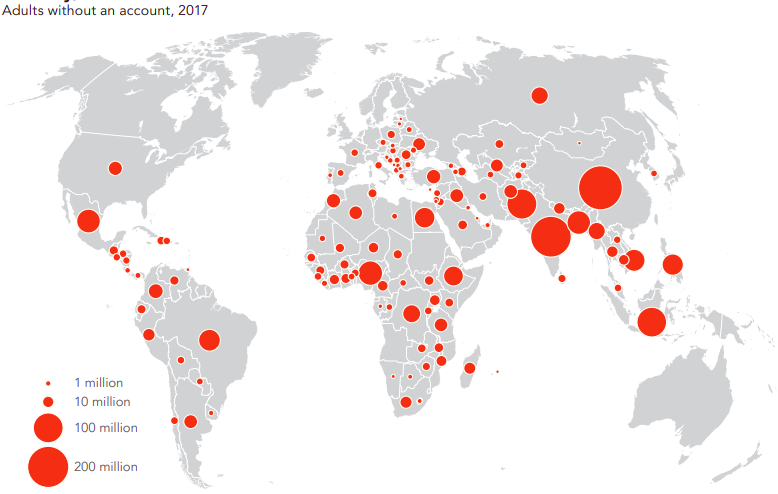
\includegraphics[width=1\linewidth]{figs/unbanked_map}
\caption{\textit{The Global Findex Database}. Map of locations for unbanked adults in 2017.}
\label{fig: unbanked_map}
\end{figure}


When looking at developing countries and financial technology (fintech) in these countries it is important to consider what is available in these areas. 1.1 billion of the financially excluded adults own a mobile phone ~\cite{gfindex}, however many developing countries have very little access to internet. Our World in Data reports that for the majority of the countries in Sub-Saharan Africa, the population with access to the internet are only between 5 and 20 percent ~\cite{owidinternet}, however for most of these countries, the mobile phone penetration rate\footnote{The mobile phone penetration rate refers to the amount of SIM cards in a certain country} is greater than 40 percent. ~\cite{owidinternet}

This paper... {\color{purple}To be continued describing what the purpose of this thesis is and what the different sections will cover}

\subsection{Potential additional topics in the introduction}
\begin{itemize}
    \item {\color{purple} An introduction and a definition of mobile payments and which types (B2B, B2C), (micro, macro)}
    \item {\color{purple} Some history of payment methods}
    \item {\color{purple} How big of a market is the mobile payment market}
\end{itemize}





% Intended learning objectives?


\section{Background and Related Work}
\subsection{Analyzis of existing secure mobile payment protocols}
For the following existing protocols: SET, iKP, KSL, LMPP, LPMP, MSET, SAMPP, SLMPP, MPCP, MPCP2, PCMS
\begin{itemize}
    \item Define them and a brief introduction to how they work
    \item Features (Do they implement the basic e-payment requirements. Refer to ~\cite{epayment_requirements})
    \item Performance (A mobile phone has to perform as few operations as possible). Refer to ~\cite{mpp_comparisons}
\end{itemize}

\subsection{Analyzis of existing mobile payment services}

\section{Proposed architecture}
\subsection{Design}
\begin{itemize}
    \item Define how its supposed to work
    \item Reason for protocol choice
    \item Reason how it ensures ACID properties
    \item Reason its fault tolerant
    \item Reason that it handles eventual consistency and asynchronous transactions
\end{itemize}

\subsection{Requirements}
As defined by ~\cite{epayment_requirements} and how they're met.
\subsubsection{Client requirements}
\begin{itemize}
    \item Usability
    \item Flexibility
    \item Affordability
    \item Reliatbility
    \item Speed of transactions
    \item Availability
\end{itemize}
\subsubsection{Server requirements}
\begin{itemize}
    \item Confidentiality
    \item Data integrity
    \item Authentication of all the participants
    \item Non-repuditian
\end{itemize}

\subsection{Implementation}

\section{Results}
How good is this implementation? Does it execute quickly, does the utilized protocol use as few operations as possible
\subsection{Findings}
\subsection{Comparison with other mobile payment platforms}

\section{Discussion}
\section{Conclusion}
\section{Future work}

\begingroup
\let\cleardoublepage\clearpage
\bibliographystyle{amsalpha}
\bibliography{thesis}
\endgroup
\end{document}